\section{Evaluation}
\subsection{Datasets}
 Both real-world and synthetic datasets were used to evaluate and compare the approximate Monte Carlo method to the standard PageRank method. The real-world datasets were obtained from the Stanford Network Analysis Project (SNAP), a well-known repository of large graph datasets \cite{standford_university_snap_2025}. It includes social networks, web graphs, and communication networks, among others. These datasets such as wiki-Talk are publicly available and can be downloaded from the SNAP website. These graphs have realistic structures with millions of nodes and edges. \par
Furthermore, synthetic graphs of any size and with different characteristics can be generated. In the experiments, Erdős–Rényi graphs of different sizes, ranging from $100.000$ to $20$ million nodes, have been generated. To establish comparable conditions between the different graph sizes, the density is kept consistent by controlling the number of outgoing edges per node. However, the in-degree of each node is random and ranges between $0$ and $n-1$, where $n$ is the total number of nodes. A simple python script was used to generate and store the graph structure in an edge list file.

\vspace{1.0em}
\begin{algorithm}[H]
\caption{Synthetic Graph Generator}
\KwIn{Range of node counts $[N_{\min}, N_{\max}]$, step size $\Delta N$, edges per node $E$}
\KwOut{Synthetic graph files with $E$ outgoing edges per node}

Set random seed for reproducibility\;
\For{$n \gets N_{\min}$ \KwTo $N_{\max}$ \KwStep $\Delta N$}{
  Create output file for graph with $n$ nodes\;
  \ForEach{node $u \in \{1, \dots, n\}$}{
    \For{$i \gets 1$ \KwTo $E$}{
      Select random destination $v \in \{1, \dots, n\}$\;
      \If{$v \neq u$}{
        Write edge $(u, v)$ to file\;
      }
    }
  }
  
}
\end{algorithm} 
\vspace{1.0em}

The selected datasets from SNAP vary in size, structure and density. The following table presents the chosen graphs and their characteristics: 

% include table
\begin{table}[ht]
\centering
\setlength{\tabcolsep}{6pt}
\renewcommand{\arraystretch}{1.2}
\begin{tabularx}{\linewidth}{l r r l X}
\toprule
\textbf{Dataset} & \textbf{Nodes} & \textbf{Edges} & \textbf{Type} & \textbf{Expected Behavior} \\
\midrule
wiki-Talk    & 2.4M & 5M    & Communication & Medium convergence \\
web-Google   & 875K & 5.1M  & Web Graph & Fast convergence, extreme authority \\
soc-Pokec    & 1.6M & 30.6M & Social Network & Slow convergence, distributed authority \\
web-BerkStan & 685K & 7.6M  & Web Graph & Fast convergence, dense connections \\
\bottomrule
\end{tabularx}
\caption{Benchmark datasets and expected behavior.}
\label{tab:datasets}
\end{table}



 %The real-world datasets selected from SNAP vary in size, density, and structure. Among them are:

%Wiki-Talk: A communication network from Wikipedia where a directed edge from user u to user v indicates that u has edited v’s talk page. This dataset contains millions of edges and is highly irregular, with some users having extremely high degree. It is one of the largest and most challenging graphs used in the experiments.

% Wiki-Vote: A voting network of Wikipedia users where edges represent votes cast in administrator elections. The dataset is smaller but directed, providing a good comparison for medium-sized graphs.

% Slashdot: A social network where edges represent “friend” or “foe” relationships between users. This dataset is useful because it represents a signed social graph with complex structure.

% Amazon Co-Purchasing Network: A product co-purchasing network where nodes are products and edges indicate that two products are often bought together. This dataset models a recommendation-style graph and offers a different type of degree distribution.


%\subsubsection{Data Sources of real-world Graphs}
% Description of synthetic and real-world datasets used


\subsection{Implementation in Spark}
% \subsubsection{Graph Representation with RDDs}
% \subsubsection{Adjacency List Construction}
% \subsubsection{Broadcasting for Teleportation}
% \subsubsection{Walker State Representation and Distribution}
% \subsubsection{RDD Caching, Materialization, and Unpersisting}
% \subsubsection{Repartitioning for Load Balancing}

The Monte Carlo Implementation is structured around two main components: The graph representation and the walker states. Both of them are stored in Sparks RDDs, which make them suitable for processing in a distributed system.\par

At the beginning of the program an edge list file is read to get the structure of the graph. It is stored as an RDD of directed edges. Then by grouping the outgoing neighbors of each node an adjacency list is constructed, which is one of the main RDD-based components, that is represnting the entire graph structure:

\vspace{0.5em}
\begin{lstlisting}[language=Scala, caption={Adjacency list creation}, label={lst:adjlist}]
val adjList: RDD[(Long, Iterable[Long])] = edgesRDD.groupByKey().cache()
\end{lstlisting}
\vspace{0.5em}

Additionally, an array of all vertices is required to support teleportation. This list will be distributed as a broadcasting variable to all nodes.

\vspace{0.5em}
\begin{lstlisting}[language=Scala, caption={Broadcasting Variable}, label={lst:broadcast}]
val broadcastNodes = sc.broadcast(allNodesArray)
\end{lstlisting}
\vspace{0.5em}

This mitigates costly network shuffles during every teleportation. Because the set of nodes is required in every simulation step it is cached in memory for efficient access.
A fixed number of walkers are initialized and represented in a seperate RDD. The RDD is distributed across multiple partitions to ensure efficient parallel processing and scaling when analyzing large graphs. Each entry in the RDD is a random vertex ID, representing the current vertex of a walker. In each simulation step the walker RDD is joined with the adjacency list to get all possible outgoing edges. After each walker updates its position, a new walker RDD is initialized with the updated positions. Before the previous walker RDD is explicitly unpersisted after the step is completed, the new walker RDD has to be materialized.
%\newpage
\begin{lstlisting}[language=Scala, caption={Materializing and Unpersisting Walker RDD}, label={lst:materialize}]
nextWalkersRDD.cache() 
nextWalkersRDD.count() // trigger an action to materialze RDD
walkersRDD.unpersist(blocking = false)
\end{lstlisting}
\vspace{0.5em}
This is because Spark uses lazy evaluation. It ensures that only the current walker RDD and the adjacency list occupy memory. \par
Before caching the walkers RDD in memory, repartitioning is applied to the RDD after each step. This is crucial for balanced distribution across partitions as it ensures that the number of partitions remains the same throughout the experiment. 
When processing large graphs that include nodes with high ingoing edges it prevents skews and stragglers allowing Spark to efficiently use all available cores. Managing the partitions correctly can have a significant impact on performance. 


\subsection{Experimental Framework and Automation}

% \subsubsection{Datasets: Real-World and Synthetic Graphs}
% \subsubsection{Synthetic Graph Generation}
% \subsubsection{Parameter Variation in Experiments}
% \subsubsection{Spark Cluster Setup}
% \subsubsection{Automation via Shell Scripts}
% \subsubsection{Data Collection and Visualization}

To evaluate the performance of the approximate Monte Carlo method an experimental framework was established, that aims for reproducibility. It benchmarks the Monte Carlo method and compares it to the standard PageRank method. The evaluation is focusing mainly on memory efficiency while trading off performance and accuracy. \par
% The datasets used for evaluation include both real-world and synthetic graphs. Real-world graphs such as wiki-Talk provide an irregular graph structure and millions of edges, presenting a practical use case. On the other hand, synthetic graphs of any size and with different characteristics can be generated. In the experiments, Erdős–Rényi graphs of different sizes, ranging from $100.000$ to $20$ million nodes, have been generated. To establish comparable conditions between the different graph sizes, the density is kept consistent by controlling the number of outgoing edges per node. However, the in-degree of each node is random and ranges between $0$ and $n-1$, where $n$ is the total number of nodes. A simple python script is used to generate and store the graph structure in an edge list file.

% \vspace{1.5em}
% \begin{algorithm}[H]
% \caption{Synthetic Graph Generator}
% \KwIn{Range of node counts $[N_{\min}, N_{\max}]$, step size $\Delta N$, edges per node $E$}
% \KwOut{Synthetic graph files with $E$ outgoing edges per node}

% Set random seed for reproducibility\;
% \For{$n \gets N_{\min}$ \KwTo $N_{\max}$ \KwStep $\Delta N$}{
%   Create output file for graph with $n$ nodes\;
%   \ForEach{node $u \in \{1, \dots, n\}$}{
%     \For{$i \gets 1$ \KwTo $E$}{
%       Select random destination $v \in \{1, \dots, n\}$\;
%       \If{$v \neq u$}{
%         Write edge $(u, v)$ to file\;
%       }
%     }
%   }
  
% }
% \end{algorithm} 
% \vspace{1.5em}

\par
During the experiments, the main parameters of the Monte Carlo method have been varied. The parameters include the number of walkers and the number of steps per walker. The goal was to systematically compare performance, memory and runtime across varying parameters. In the GraphX implementation the only parameters that were configured are the tolerance and the damping factor. The tolerance is usually set to $0.001$. In the experiments it was kept on such a low value to get very precise PageRank values and to compare the approximate Monte Carlo approach to the standard PageRank method. The reset probability was set to $0.15$ for both methods. Additionally, different Spark configurations were analyzed such as the number of executors and most importantly the memory allocated per executor. \par



To automate the experiments, shell scripts are used. Each script relies on spark-submit, which is the standard command line tool used to launch applications on a Spark cluster. In the spark-submit command configurations such as the number of executors and the memory per executor can be set. Furthermore, the edge list file is passed to the script as well as the Monte Carlo specific configuration such as the number of walkers and steps per walker. This setup ensures that experiments are running in a sequence without needing manual input and with consistency throughout multiple data sets. Finally, the spark-submit command allows to either run the applications locally or to launch them to a cluster environment to simulate a real distributed system. \par

\begin{figure}[H]
    \centering
    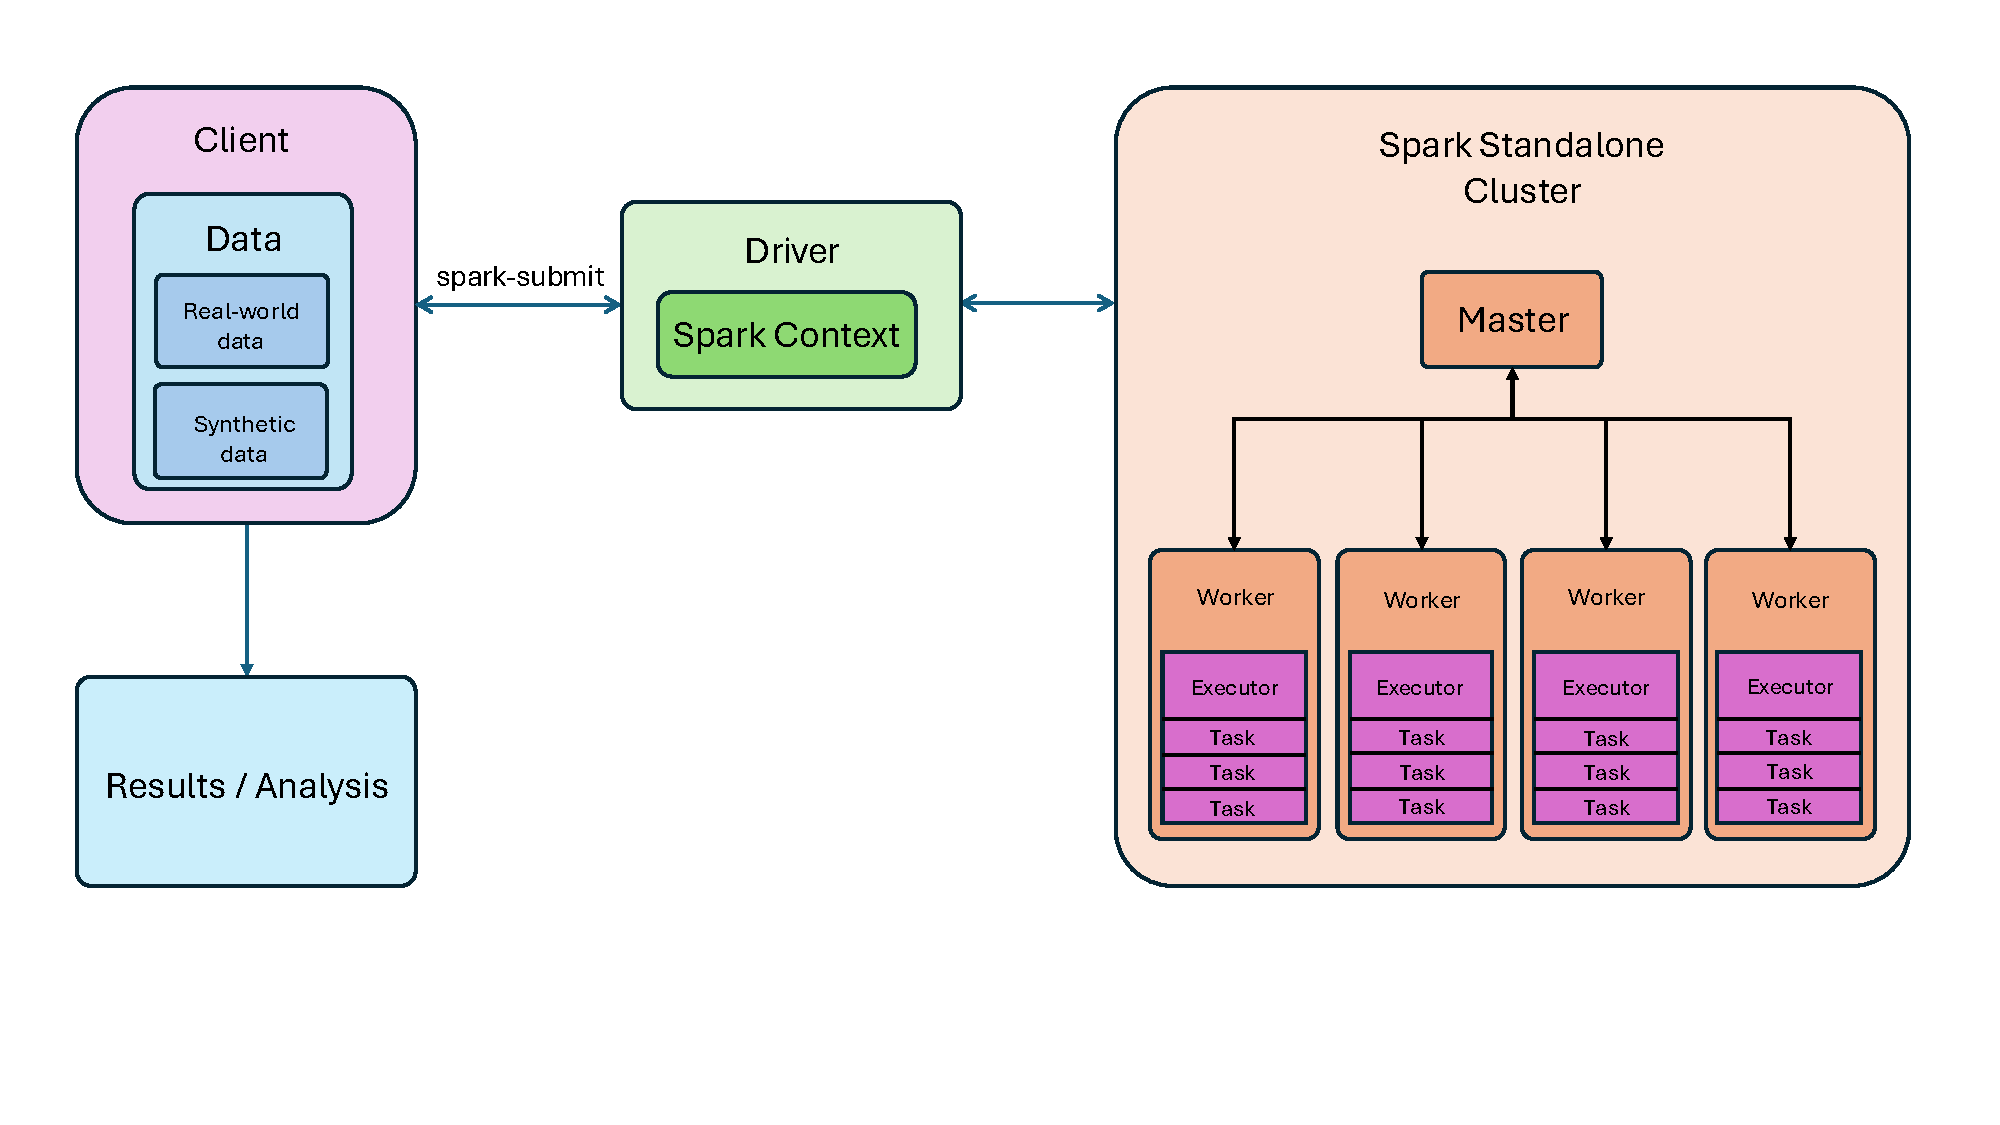
\includegraphics[width=\linewidth]{images/Workflow_image.pdf}
    \caption{Experimental Workflow}
    \label{fig:workflow}
\end{figure}
To ensure comparable conditions across all experiments, all experiments were executed on a Spark cluster set up on the university's server. For simplicity, the Spark cluster was deployed in standalone mode, which is a built-in cluster manager. Only the master and workers need to be started on the university server. The cluster consists of one master node and four worker nodes. Each worker node has one executor with two cores, for a total of eight cores. \par


In every experiment, metrics for both methods were collected, including configurations such as the number of walkers and steps for the Monte Carlo method. Another file collected the total runtime, allocated memory, and graph size to evaluate performance with limited memory and with different graph sizes. For accuracy evaluation, the top 20 ranks for both methods were saved in a separate file. \par
All the collected data was saved in CSV files to efficiently analyze it in the next step. With the help of Python scripts and the use of libraries such as Matplotlib and Pandas, the data is structured and visualized in various plots of runtime, allocated memory, accuracy and cost. This provides a clear overview of the data and enables a thorough analysis of the data. \par
This setup ensures the reproducibility and scalability of evaluating the Monte Carlo method. This was achieved through the use of various datasets, such as real-world and synthetic data, as well as a systematic variation in parameters. Additionally, scripts automated experiments and efficiently collected key metrics. This framework enabled the analysis of the empirical results presented in the following sections. \par
% \begin{figure}[H]
%     \centering
%     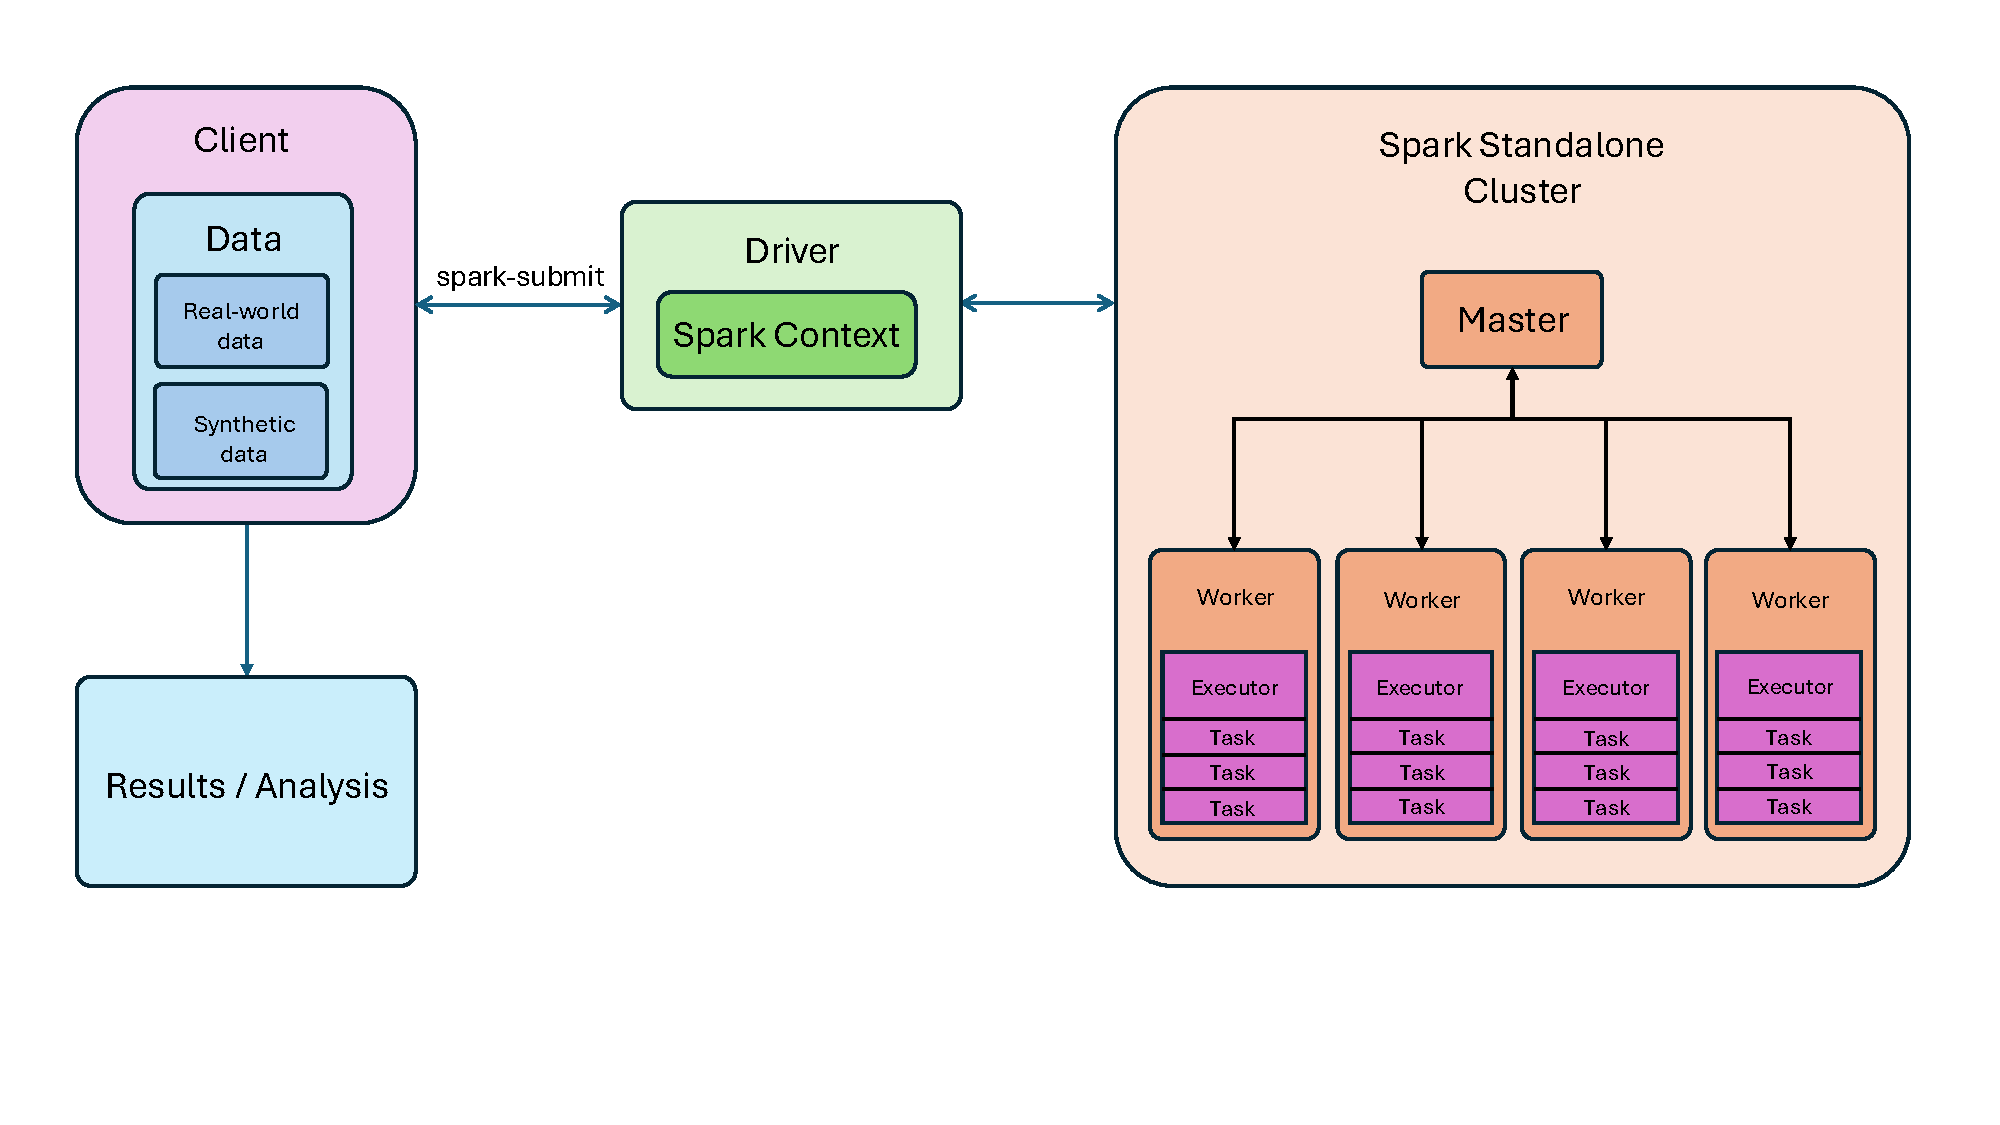
\includegraphics[width=\linewidth]{images/Workflow_image.pdf}
%     \caption{Experimental Workflow}
%     \label{fig:workflow}
% \end{figure}
Finally, the given approach combines an approximate Monte Carlo implementation with a distributed Spark environment and a systematic experimental framework. The main goal of this setup was to determine whether the described method can operate with much less memory than the standard PageRank implementation. While a trade-off in accuracy and performance was expected and tolerated, the method aims to provide sufficient accuracy and performance. The evaluation will reveal whether the Monte Carlo approach is a viable alternative to the standard PageRank method in environments with restricted memory and large-scale graphs, addressing the central research question of this thesis.


\subsection{Error Handling}
% \subsubsection{Out-of-Memory Handling}
% \subsubsection{Crash Scenarios Encountered During Experiments}
% \subsubsection{Timeout: How and when to cancel an Experiment}

When processing large-scale graphs, memory exhaustion and application crashes are inevitable. Therefore, error-handling strategies were necessary to ensure that experiments remain reproducible and manageable. For simplicity, this thesis only differentiates between out-of-memory (OOM) failures and timeouts. \par
The Java Out-of-Memory exception is a common scenario that was expected in this experimental setup because the goal was to deliberately strain memory. This exception is usually thrown when there is not enough memory in the Java heap to allocate to an object. This means the garbage collector is unable to free up enough space for the object. In these experiments, the exception was detected in the log files. In that case, the configurations were automatically marked as failed and excluded from further experiments. \par
Since very large graphs were being processed, some experiments can take a disproportionately long time to finish. This is why a timeout mechanism was implemented to prevent experiments from blocking the pipeline. If an experiment did not finish within the predefined time, the current experiment was terminated, and the next experiment with different configurations started. This ensures that all experiments finished within an acceptable time frame.  \par
These error handling strategies established a more systematic and stable process. Experiments could run without manual intervention, and the resulting datasets are more consistent.

% \subsection{Datasets}
 


% \subsubsection{Data Sources of real-world Graphs}
% % Description of synthetic and real-world datasets used.

\subsection{Allocated Memory}
The main goal of this thesis was to investigate wether the Monte Carlo PageRank approach is able to operate on restrained memory and compare it to the standard PageRank approach. Therefore, allocated memory was analyzed as the key evaluation metric. 
\vspace{0.5em}
\begin{lstlisting}[language=bash, caption={Spark-submit command}]
spark-submit \
  --class "$SPARK_APP_CLASS" \
  --master spark://casa-ubu.eecsit.tu-berlin.de:7077 \
  --name "Demo-$base-$EXECUTOR_MEM" \
  --deploy-mode client \
  --driver-memory 3g \
  --executor-cores 2 \
  --conf spark.cores.max=8 \
  --executor-memory "$EXECUTOR_MEM" \
\end{lstlisting}
\vspace{0.5em}
In Spark, the executor memory is allocated through spark-submit, which is shown above. The parameter executor-memory specifies the available JVM heap size per executor. For all experiments the allocated memory per executor was varied and set between 450 MiB and 8 GiB. Other parameters such as the number of executors and total numbers of cores were kept the same to ensure comparability throughout all experiments.\par
The memory configurations were logged for both the Monte Carlo method and the standard method. In case the allocated memory was not sufficient for the application and an OOM exception was thrown, the error was handled as mention above. The failed runs show the boundaries of each method under limited memory. The focus of the analysis is put on the minimum memory required and how this changes with increasing the graph size. The results are compared between the two methods. \par





\subsection{Runtime}
Runtime is another metric that was analyzed in this thesis. It shows how both methods perform under limited memory conditions. Although a trade-off in runtime was considered as acceptable, the methods should aim to finish within an acceptable time under the given circumstances. It also shows the practicality of both methods.\par
Therefore, a timeout of 30 minutes was implemented and the experiments were handled according to the error handling section.\par 
The total runtime of each experiment was measured from when the Spark application was submitted until the Spark Session was stopped. The shell scripts that automated the experiments also logged the runtime and the configurations, which ensures an identical setup across all experiments.\par
The analyses focuses mainly on the effect of different graph sizes on the runtime. 


\subsection{Accuracy}
The accuracy was evaluated by comparing the ranks of the Monte Carlo method and the standard PageRank method. The standard PageRank method is considered to be the ground truth as it was configured with a tolerance of $0.001$. During the experiments the goal was to determine how close ranks are to the ground truth. Accuracy is mainly controlled by the number of walkers, the steps per walker and the graph structure. \par

Since in many real-world applications only require the top ranks are needed, the goal was to only analyze the top $20$ ranks. The ranks were also collected through the shell scripts. The accuracy was then determined by the Jaccard index, which is a statistic used to measure the similarity and distance of sample sets. Jaccard index in combination with the top $20$ ranks is very simple and focuses on overlap of important nodes instead of overemphasizing tail nodes.

\vspace{1.0em}
\begin{algorithm}[H]
\caption{Jaccard Similarity}
\KwIn{Two rank lists $L_{MC}$, $L_{GX}$}
\KwOut{Similarity $s$, Distance $d$}

$S_{MC} \gets$ set($L_{MC}$) \;
$S_{GX} \gets$ set($L_{GX}$) \;

$I \gets |S_{MC} \cap S_{GX}|$ \;  
$U \gets |S_{MC}| + |S_{GX}| - I$ \; 

$s \gets I / U$ \;
$d \gets 1 - s$ \;

\Return $(s, d)$ \;
\end{algorithm}
\vspace{1.0em}

The resulting value is a percentage that represents the similarity to the ground truth. \par

The accuracy was analyzed on different graph sizes and structures. Additionally the number of walkers and the number of steps was varied across experiments. With an increasing number of walkers and steps a higher accuracy was expected. Furthermore larger and more complex graphs would require more walkers to achieve good accuracy. Also, a variance in the ranks of the Monte Carlo approach was expected since it follows the random surfer model and identical ranks are unlikely. Therefore, the average similarity of the top $20$ ranks across five different runs with the same configurations was taken to get a more representative result.


\subsection{Costs (GiB-hours)}
% Memory usage, runtime, accuracy (e.g., compared to GraphX).
A cost metric was introduced to reflect both runtime and minimal allocated memory. GiB-hours combines these two metrics to show how much cluster memory was allocated and for how long. It is the area under the memory time curve. For each experiment, it was computed by multiplying the allocated executor memory (GiB) by the runtime (hours). \par
Since the setup was constant across all experiments, the cost metric was primarily influenced by executor memory and runtime. The driver memory was also kept constant to maintain focus on executor memory during the experiments and to make to GiB-hours directly comparable across Monte Carlo and GraphX experiments. Additionally, no off-heap or reserved memory was added. Thus, the cost metric depends solely on the configured on-heap executor memory. However, GiB-hours doesn't capture all costs such as the network costs.\par
If only the runtime had been taken into account, the experiments with high memory demand would have appeared to be more favorable, even though they consumed much more memory. This is why the cost metric is crucial for providing a balanced overview. It captures both runtime and memory usage during the experiment. \par
The analysis predicted that the Monte Carlo approach would require fewer GiB-hours, while the standard PageRank method was expected to be significantly more costly.


\subsection{Results and Plots}

\subsubsection{Performance}

The performance experiments show how the Monte Carlo and the GraphX implementation perform under different memory constraints and graph sizes. The first two plots show the executor versus runtime behavior of both methods on real-world graphs. \par
The first plot is based on the \textbf{Wiki-Talk} Graph. This dataset represents a communication network with 2.4 million nodes and 5 million edges. It is the therefore the largest graph used across the experiments. Although, both methods perform very similar, the GraphX method encounters out-of-memory and timeout errors under 2000 MiB, while the Monte Carlo method successfully finishes at all memory configurations. The total runtime of all successful runs stays under 200 seconds, where the Monte Carlo almost remains constant at 100 seconds and the GraphX method starts around 170 seconds and then aligns with the Monte Carlo method. This proves the superior ability of the Monte Carlo approach to operate under very restricted memory conditions.\par
The second plot shows the performance on the \textbf{Web-Google} graph, which is a web graph with 875K nodes and 5.1 million edges. A very noticeable difference to the wiki-Talk plots can be observed in the performance plot, where the strengths of the Monte Carlo method can be seen. The Monte Carlo method keeps runtimes consistent under 100 seconds across all memory configurations, which suggests that the the memory consumption stays well within the available resources.However, the GraphX method requires a lot more time to finish under memory pressure with a total runtime of 1300 seconds at 700 MiB per Executor. As allocated memory increases the performance of the GraphX method improves drastically and stabilizes at comparable runtimes as the Monte Carlo method. The extreme authority, typical for web-graphs, appears to cause the bad performance of the GraphX method under memory pressure. This is likely caused by excessive garbage collection triggered by the GraphX matrix multiplication that is operating with limited memory. Whereas the Monte Carlo approach with it's fixed number of walkers avoids that problem entirely since the memory footprint is proportional only to the number of walkers. \par




\begin{figure}[H]
    \centering
    \begin{subfigure}[t]{0.5\linewidth}
        \centering
        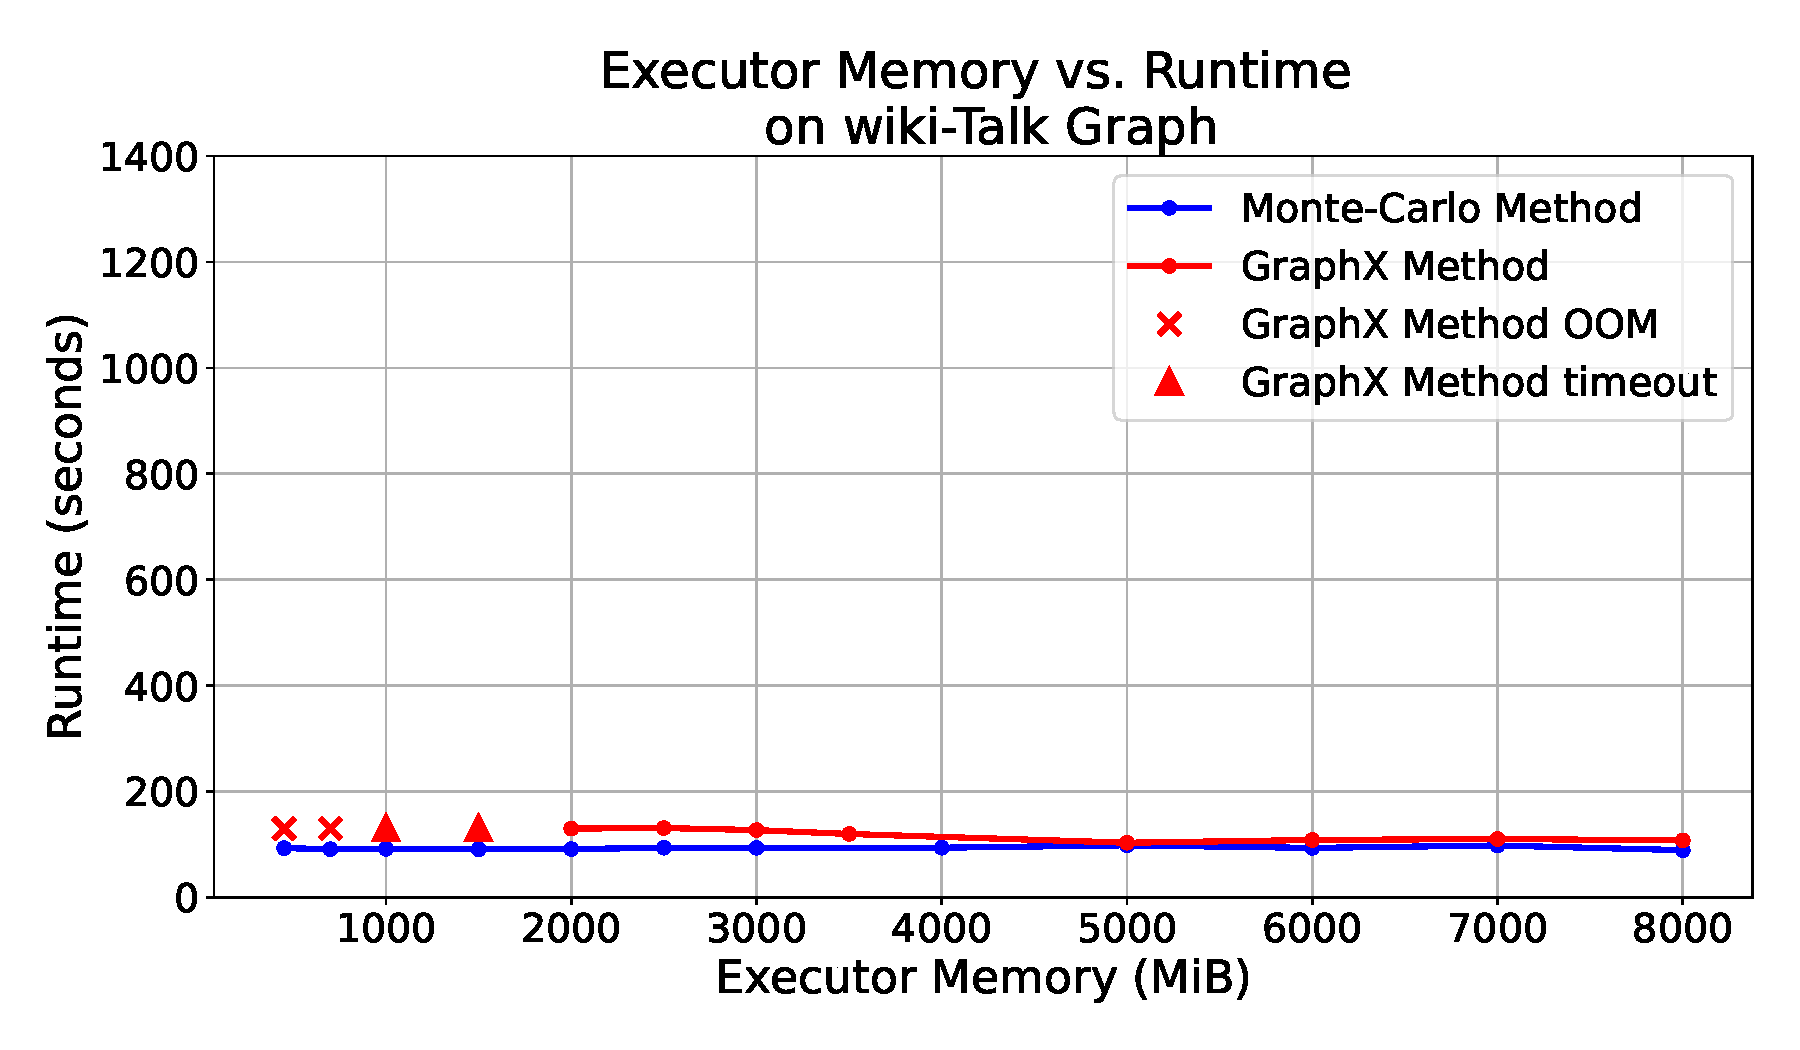
\includegraphics[width=\linewidth]{images/plots/wiki-Talk/memory_vs_runtime_wiki_talk.pdf}
        \caption{Wiki-Talk Graph}
        \label{fig:wikirun}
    \end{subfigure}\hfill
    \begin{subfigure}[t]{0.5\linewidth}
        \centering
        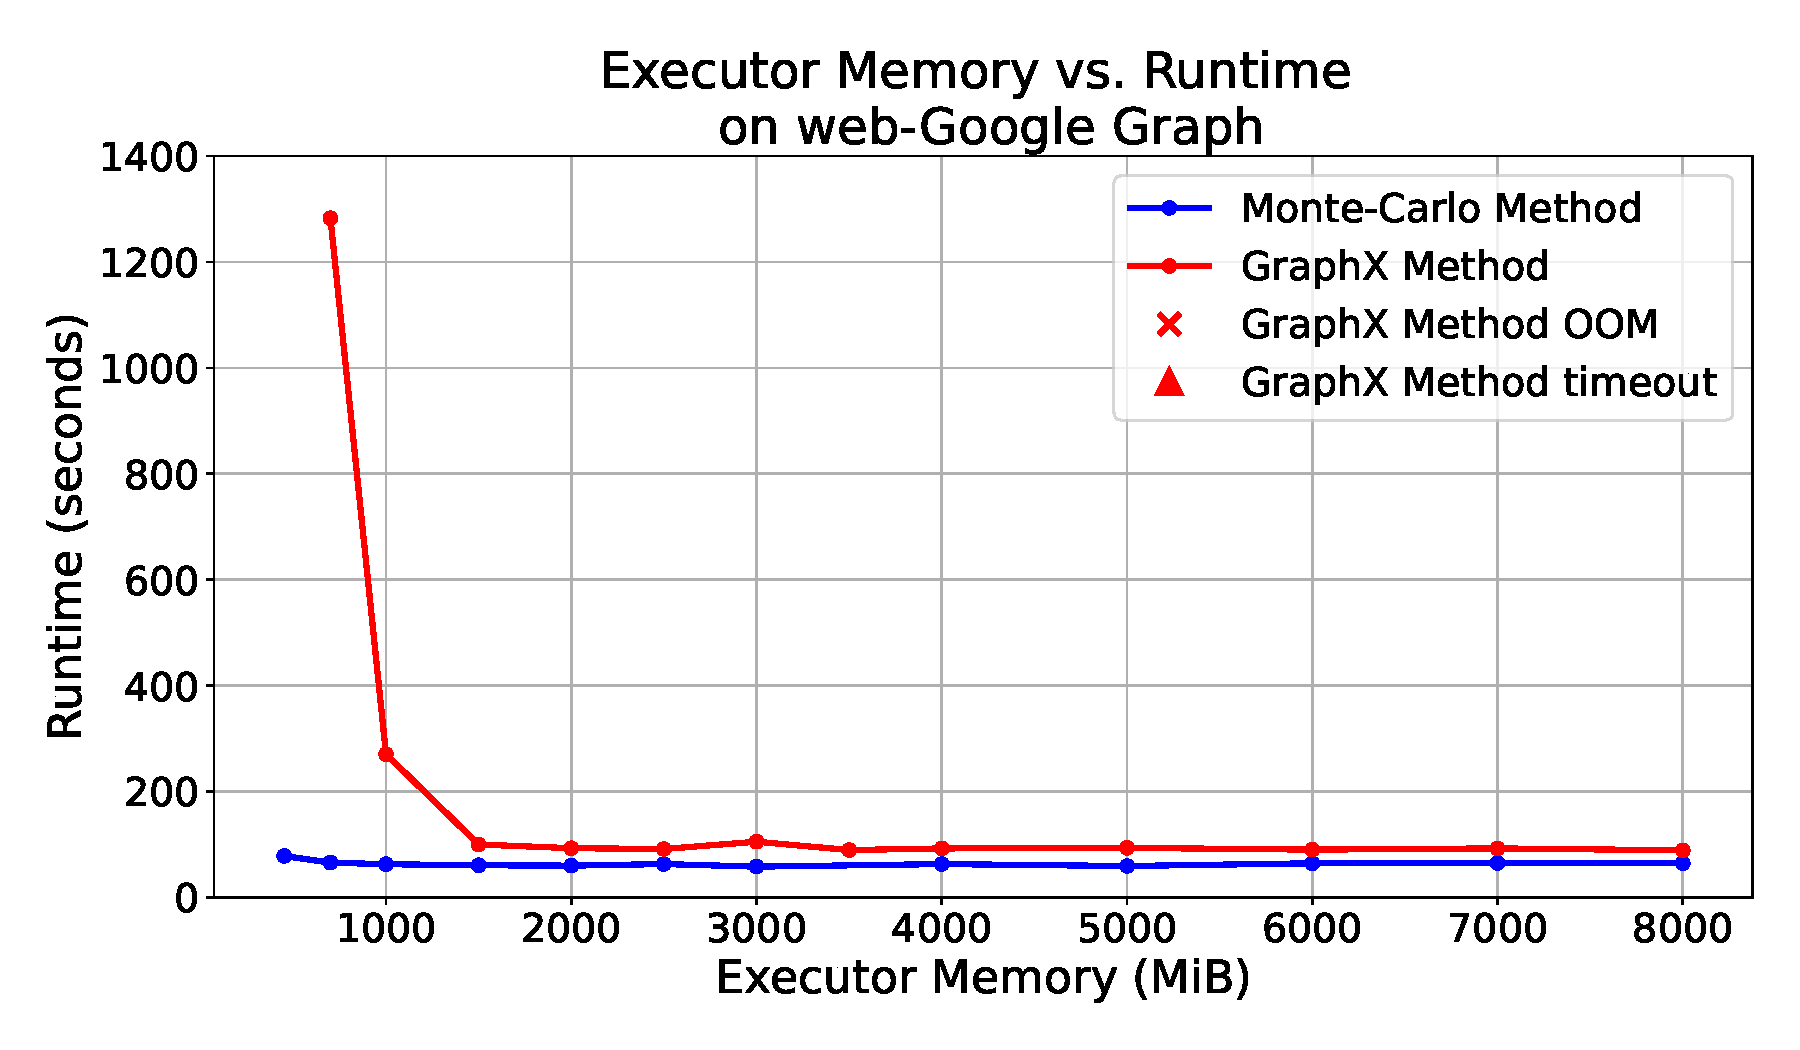
\includegraphics[width=\linewidth]{images/plots/web-Google/memory_vs_runtime_web_google.pdf}
        \caption{Web-Google Graph}
        \label{fig:wikigibhrs}
    \end{subfigure}
    \caption{Memory vs. Runtime}
    \label{fig:wiki-comparison}
\end{figure}

The following plots show the performance of both methods on synthetic Erdős-Renyi graphs. The analysis gives an insight on how the methods perform with increasing graph size while keeping the same graph structure.\par
The analysis of the ER graph with two edges per node includes the runtime and the minimal memory configuration used for that graph size. For the Monte Carlo method, the runtime starts below 100 seconds at 100 thousand nodes and then increases to just under 1500 seconds at 20 million nodes. During the experiments the required memory remains stable at 450 MiB. The GraphX method's runtime starts similar to the Monte Carlo method but then has higher runtimes for graphs between 200 thousand and 800 thousand nodes. However, for graphs between 900 thousand and 20 million nodes the runtimes of the GraphX method are lower compared to the Monte Carlo method. Although the performance of the GraphX method is better on bigger graphs the required memory is much higher than in the Monte Carlo method. GraphX starts with 450 MiB on the smallest graph but quickly increases to 3000 MiB and then finally to 8000 MiB at 20 million nodes.\par
When increasing the edge count per node to three, the memory differences between the methods become clearer. While both methods perform similar compared to the previous experiment, the GrapX method has a timeout at 20 million nodes. The required memory for the Monte Carlo method remains at 450 MiB across all graphs. In contrast, the GraphX method's memory increases starting from 450 MiB to 6000 MiB at 1 million nodes and 8000 MiB at 15 million nodes.\par
The performance analysis reveals different key findings. First, the Monte Carlo method demonstrates much better performance stability under constraint memory, while GraphX either fails or suffers from poor performance. Second, the graph structure has a significant influence on the performance. Web graphs with extreme authority show most advantages for the Monte Carlo method, while more balanced communication graphs like wiki-talk only show little advantage of the Monte Carlo method. Lastly, the Monte Carlo method encounters much better scalability on large graphs, maintaining a low memory consumption, while GraphX requires a much higher amount of memory. The performance experiments show that the Monte Carlo method is superior to standard methods as it is able to operate in a memory constrained environment without trading off performance.


\begin{figure}[H]
    \centering
    \begin{subfigure}[t]{0.5\linewidth}
        \centering
        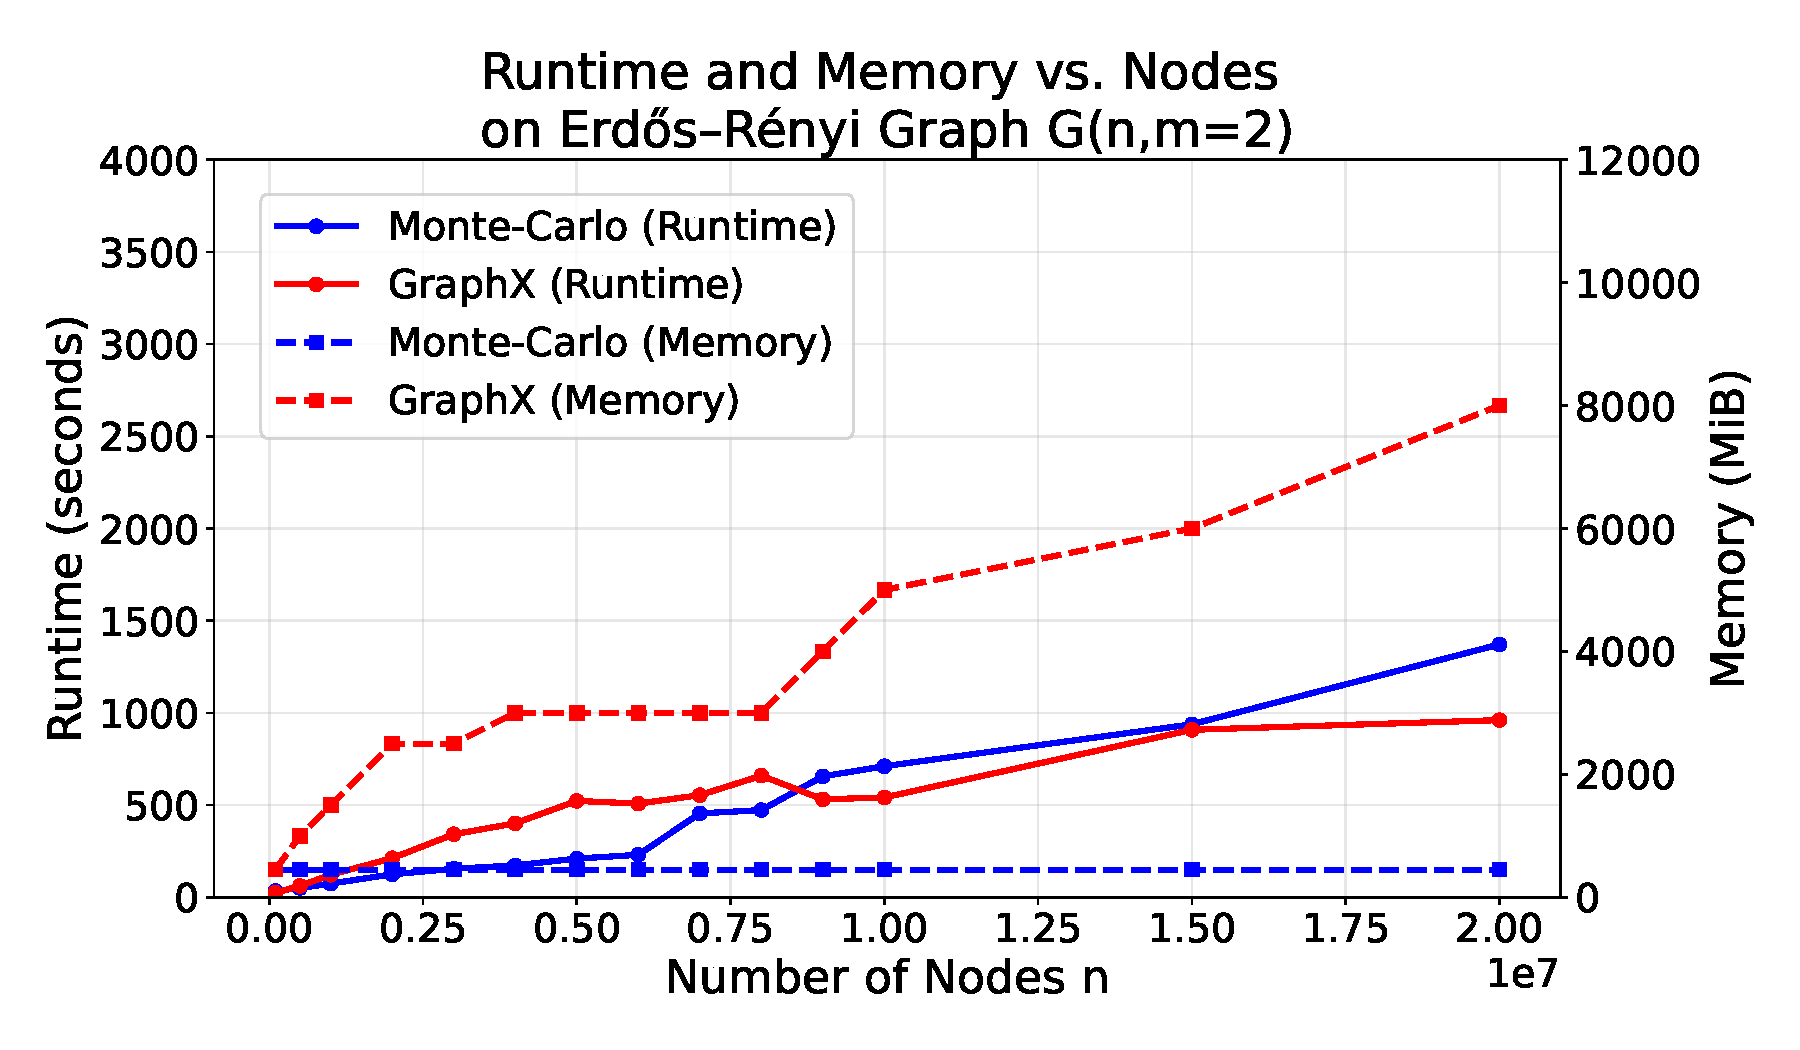
\includegraphics[width=\linewidth]{images/plots/ER_2edg/combined_runtime_memory_vs_nodes_2edges_gx_mc.pdf}
        \caption{Erdős–Rényi Graph with two outgoing edges per node}
        \label{fig:wikigibhrs}
    \end{subfigure}
    \begin{subfigure}[t]{0.5\linewidth}
        \centering
        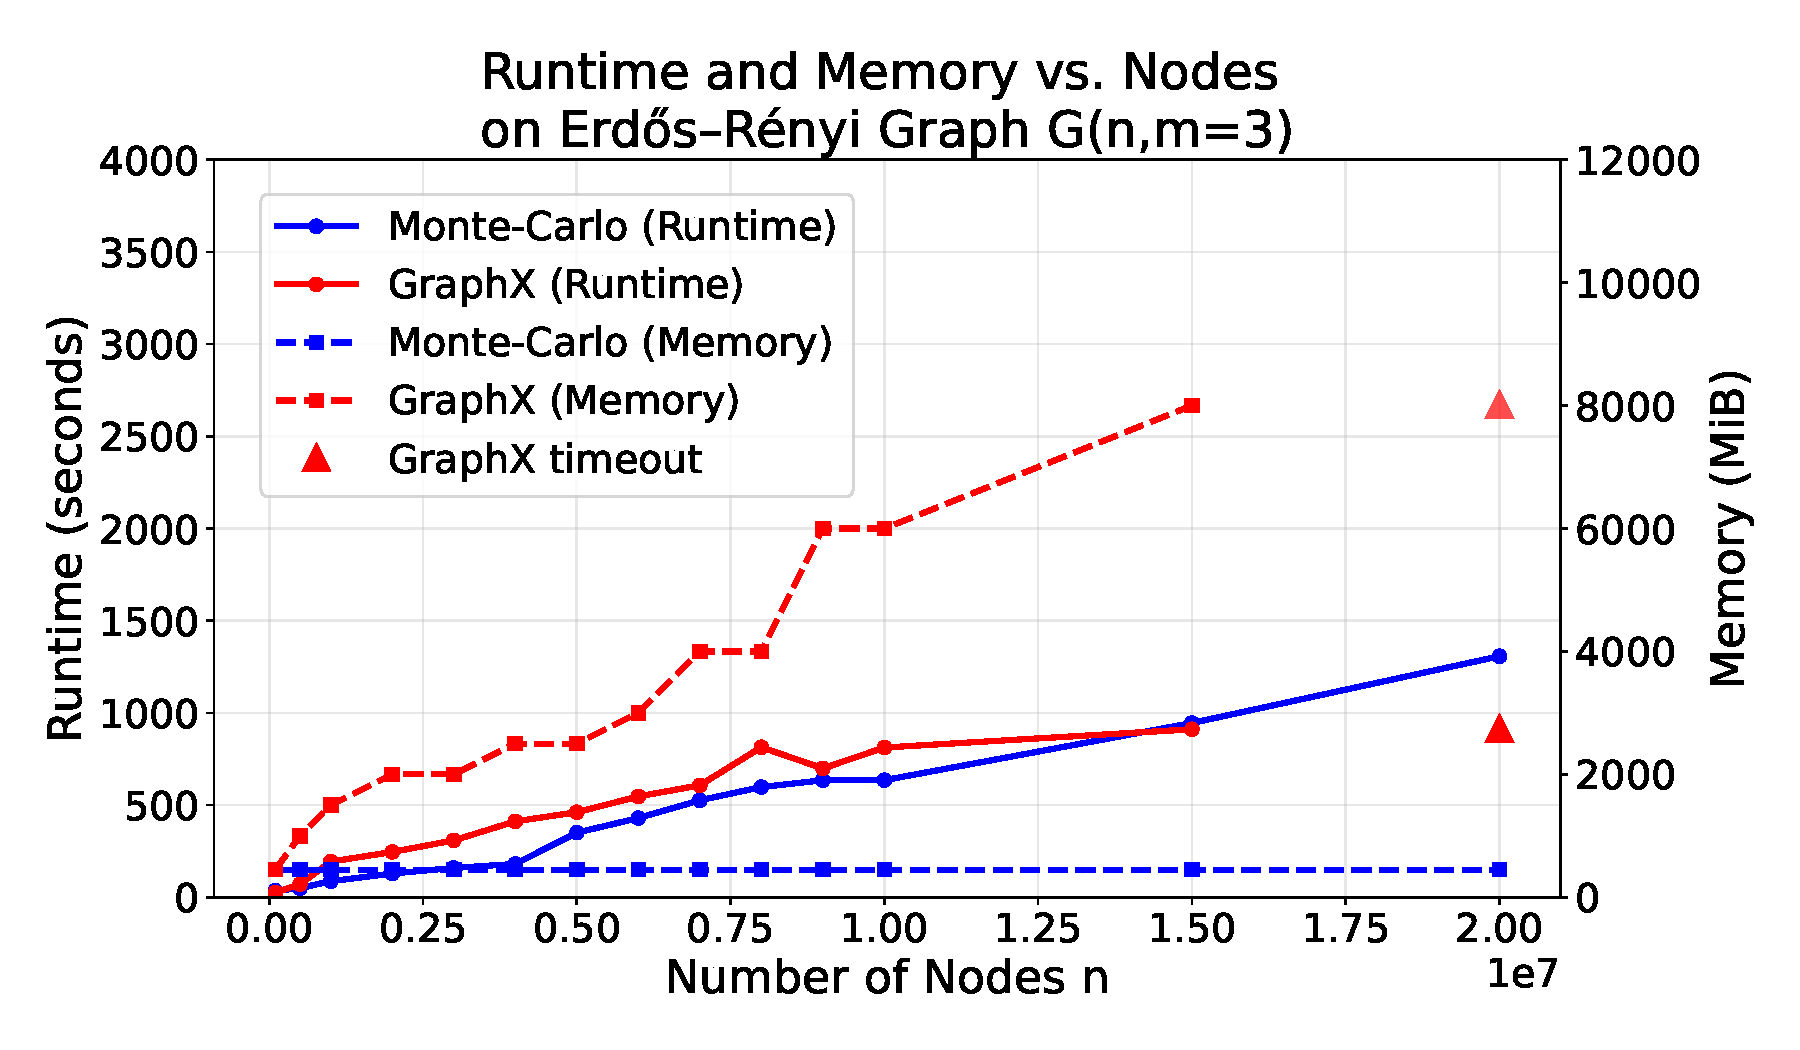
\includegraphics[width=\linewidth]{images/plots/ER_3edg/combined_runtime_memory_vs_nodes_3edges_gx_mc.pdf}
        \caption{Erdős–Rényi Graph with three outgoing edges per node}
        \label{fig:wikigibhrs}
    \end{subfigure}
    \caption{Performance Graphs}
    \label{fig:wiki-comparison}
\end{figure}



%synthetic plots runtime
\subsubsection{Costs}
%real world plots cost
\textbf{Wiki-Talk.} The cost experiment on the wiki-talk shows that the Monte Carlo method is less costly over all. The Monte Carlo method nearly shows a linear line that is starting just above zero and then rises to 0.2 GiB-hours. The GraphX method encounters out-of-memory and time-out errors for smaller memory configurations like already observed in the performance plot. For memory configurations between 2000 MiB and 8000 MiB, the GiB-hours are similar to the Monte Carlo method. This linear relationship of the Monte Carlo method shows the consistent runtime across different memory configurations.\par

\textbf{Web-Google.} The experiments on the web-Google graph reveal a bigger cost difference between the two methods. Again, the Monte Carlo method's cost analysis shows a linear line with lower GiB-hour values compared to the wiki-Talk graph. At 8000 MiB the cost are 0.15 GiB-hours. The GraphX method is much more costly for lower memory configurations as the total runtime is significantly higher than for higher memory configurations. GraphX has a peak at 700 MiB with 0.25 GiB-hours and then decreases to 0.05 GiB where it almost aligns with the Monte Carlo method and rises again to 0.2 GiB at 8000 MiB. \par





\begin{figure}[H]
    \centering
    \begin{subfigure}[t]{0.5\linewidth}
        \centering
        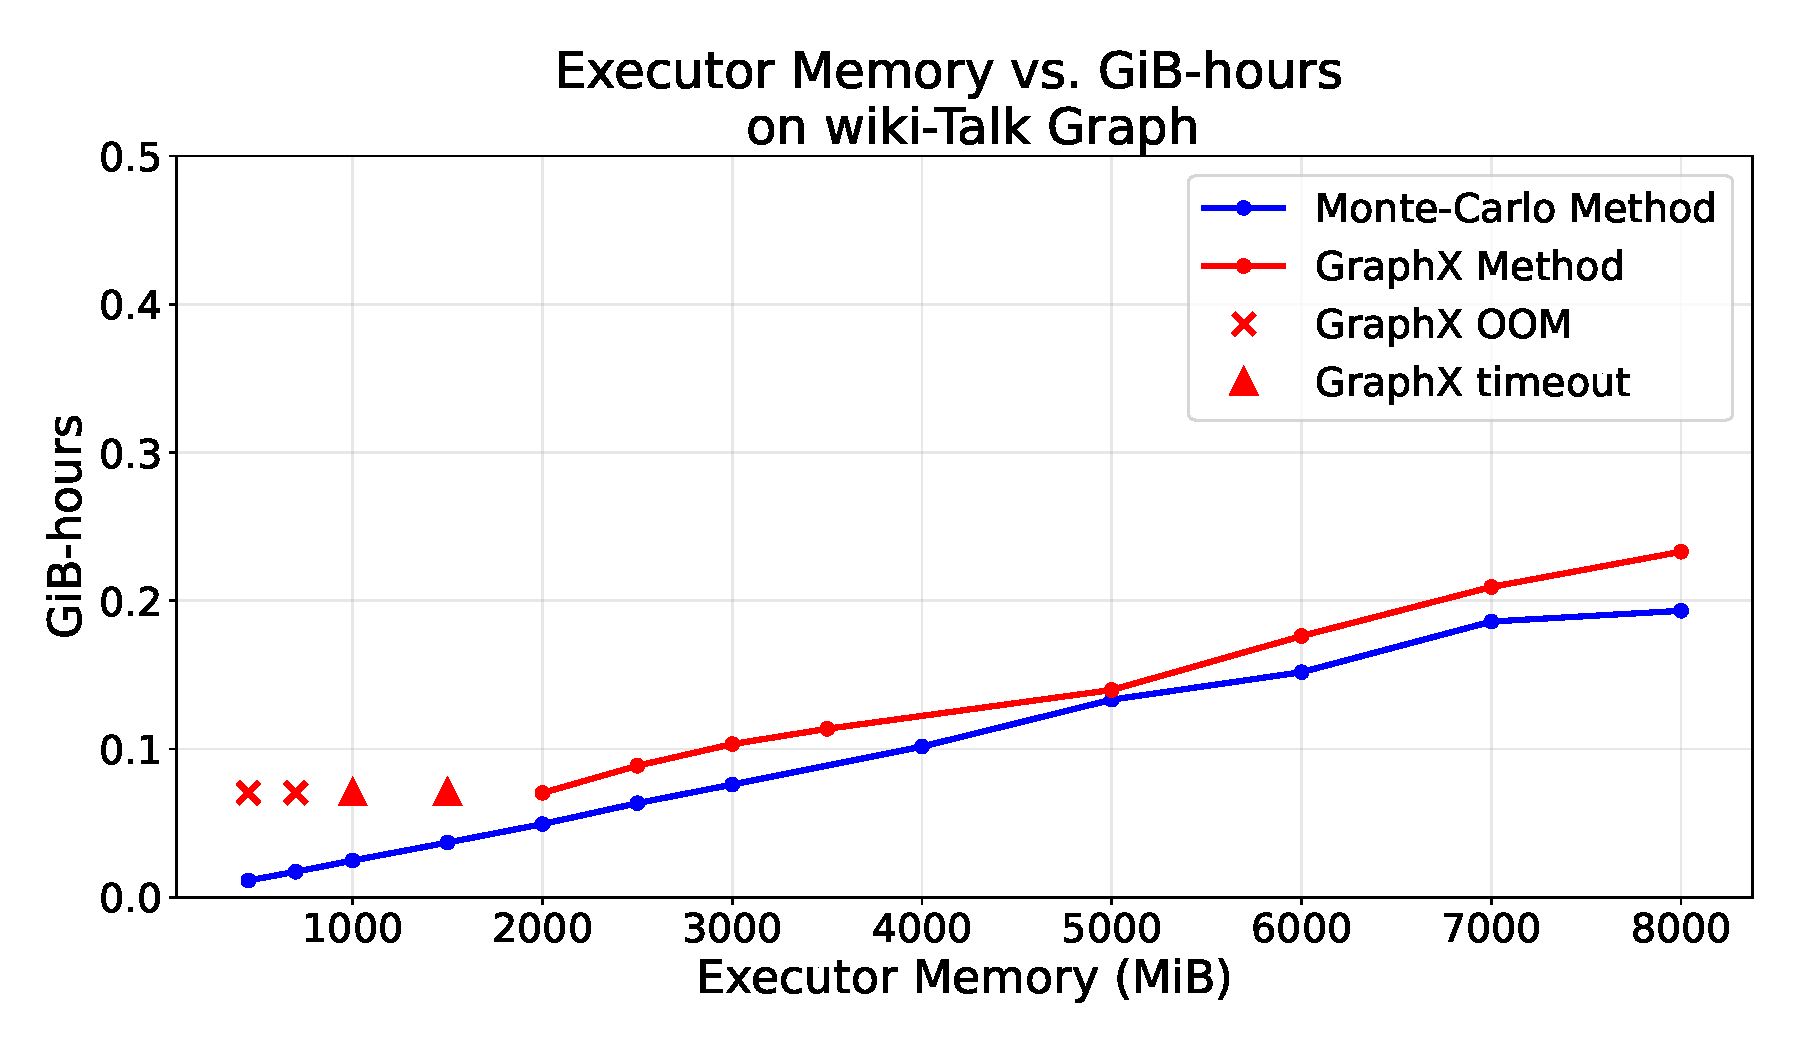
\includegraphics[width=\linewidth]{images/plots/wiki-Talk/gbhrs_nodes_wiki_talk.pdf}
        \caption{wiki-Talk Graph}
        \label{fig:wikirun}
    \end{subfigure}\hfill
    \begin{subfigure}[t]{0.5\linewidth}
        \centering
        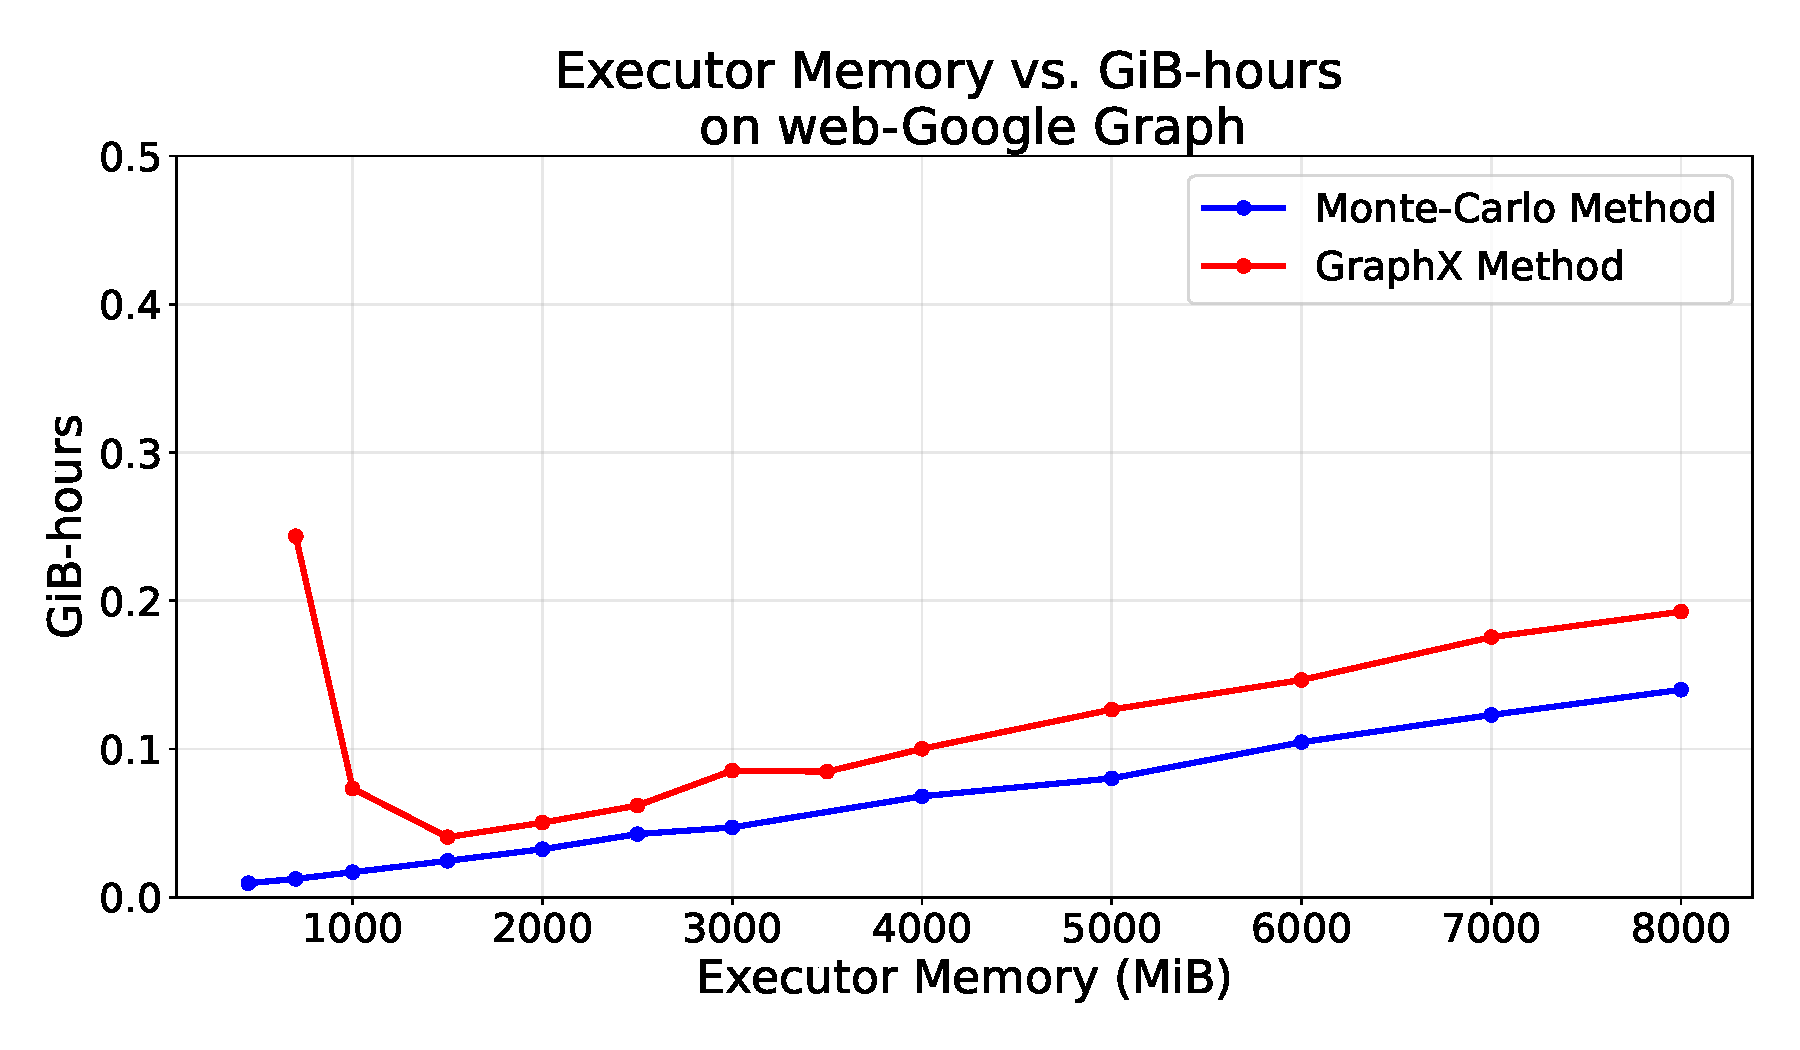
\includegraphics[width=\linewidth]{images/plots/web-Google/gbhrs_nodes_web_google.pdf}
        \caption{web-Google Graph}
        \label{fig:wikigibhrs}
    \end{subfigure}
\end{figure}


The cost graph based on an synthetic ER graph with two edges per node reveals a clear behavior of both methods. The Monte Carlo method remains on a stable cost level with a maximum of 0.25 GiB-hours at 20 million nodes. GraphX on the other hand demonstrates significantly higher costs on larger graphs. It is starting from a similar level as the Monte Carlo method just above zero but then rapidly increases to over 2 GiB-hours at 20 million nodes.\par
The analysis of teh ER graph with three edges per node shows a very similar behavior. While the Monte Carlo method remains on a stable level with a maximum of 0.25 GiB-hours, GraphX reveals a steeper curve compared to the analysis on the ER with two edges per node. It reaches it's maximum at 15 million nodes with 2 GiB-hours. Another difference to the graph above is that GraphX encounters a timeout at 20 million nodes. \par
The cost analysis reveals that the Monte Carlo method provides significant economic advantages across different graph sizes and structures. 
For real-world graphs with irregular structures such as the web-Google graph, the costs of the Monte Carlo method stays consistently low and predictable. GraphX on the other hand, either encounters very high costs or failures under constraint memory.\par
The analysis on synthetic graphs reveals even more the cost advantage. While the Monte Carlo method remains at a stable low level, GraphX costs escalate and encounters scalability issues as computations fail to complete. \par
These findings have significant impact on real world deployment scenarios where computing environments get billed based on memory allocation and time. The lower GiB-hours of the Monte Carlo method result in lower operational costs. Moreover, the ability of the Monte Carlo method to successfully complete with limited memory allow the processing of large graphs that would be otherwise infeasible due to high costs. Additionally, the stable behavior of the Monte Carlo approach enables better resource planing compared to the unpredictable behavior of the GraphX approach.


\begin{figure}[H]
    \centering
    \begin{subfigure}[t]{0.5\linewidth}
        \centering
        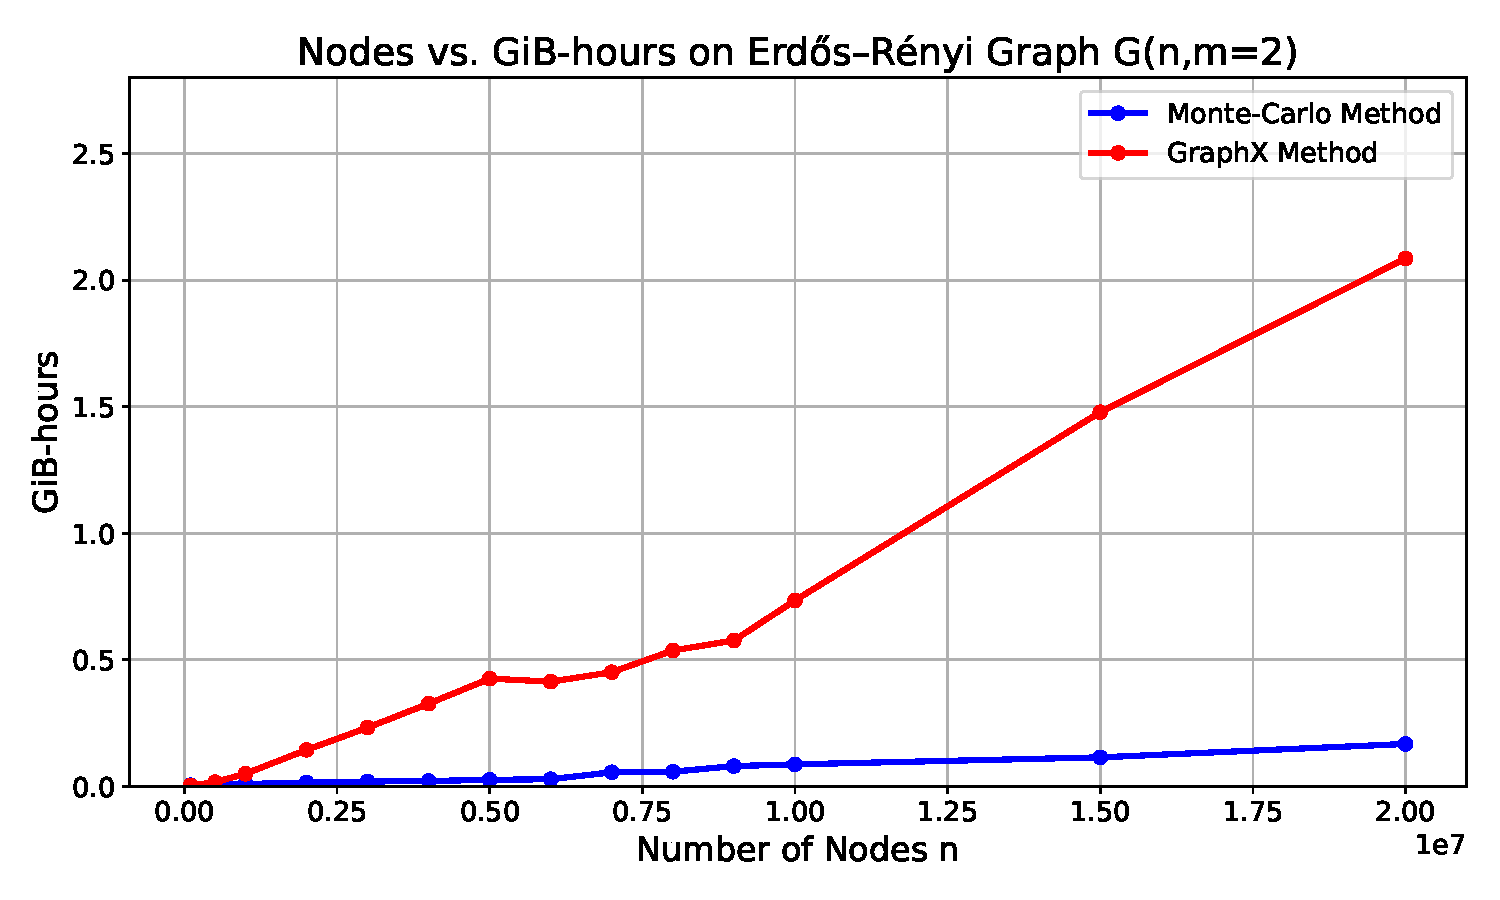
\includegraphics[width=\linewidth]{images/plots/ER_2edg/gbhrs_nodes_er_graph_2edges.pdf}
        \caption{Erdős–Rényi Graph with two outgoing edges per node}
        \label{fig:wikigibhrs}
    \end{subfigure}
    \begin{subfigure}[t]{0.5\linewidth}
        \centering
        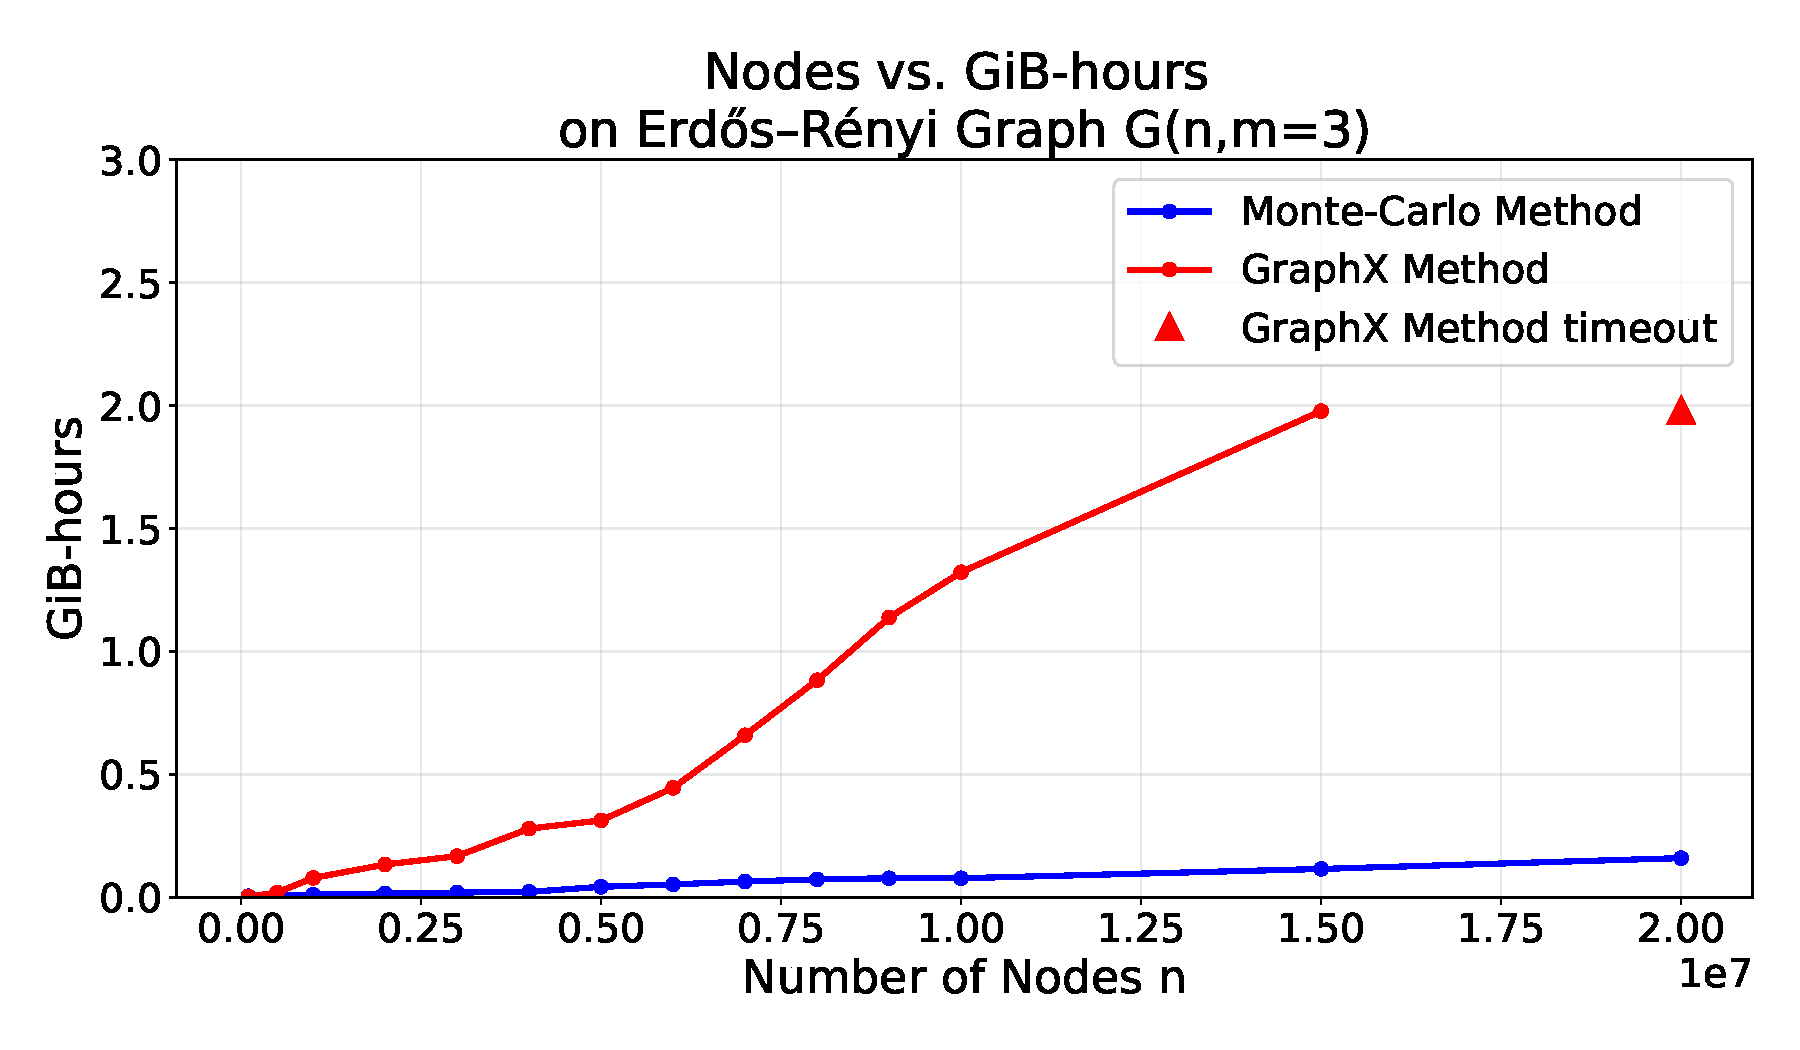
\includegraphics[width=\linewidth]{images/plots/ER_3edg/gbhrs_nodes_er_graph_3edges.pdf}
        \caption{Erdős–Rényi Graph with three outgoing edges per node}
        \label{fig:wikigibhrs}
    \end{subfigure}
    \caption{Cost Graphs}
    \label{fig:wiki-comparison}
\end{figure}

%synthetic plots costs
\subsubsection{Accuracy}
%real world plots accuracy

\textbf{Wiki-Talk.} The accuracy analysis for the wiki-Talk graph shows strong performance of the Monte Carlo method across different walker configurations. The plot analyzes the Jaccard similarity between varying walker configurations. All experiments use 10 steps per walker and a reset probability of 0.15. Overall the Monte Carlo method achieves accuracy scores above 80\%. Even with the minimal amount of one walker per node, the Monte Carlo method achieves a similarity of 83\%, meaning that 83\% of the top 20 nodes determined by the Monte Carlo method overlap with the ones of the GraphX method. With an increasing number of walkers the accuracy only improves at a really low rate. At the maximum configuration in this experiment of five walkers per node the similarity reaches 85\%. It can also be observed that the accuracy curve flattens after two walkers per node, which suggests an effective convergence in the communication network with only a small amount of walkers. This indicates that walker configurations over two to three walkers don't return into significant higher accuracy and therefore configuring three walkers at most guarantees sufficient accuracy.\par
The high accuracy scores can be explained with the typical structure of communication networks, which typically have a more balanced degree distribution than web graphs. Therefore, only a few random walkers are required to effectively explore the entire graph structure. This suggests that for real-world applications the most resource efficient configuration of one walker per node achieves relatively high accuracy.\par
\textbf{Web-Google.}The web-Google graph presents a more challenging scenario for approximating PageRank with the Monte Carlo method. This is because of it's extreme authority structure that is typical for web graphs. With the minimum of one walker per node the method achieves a 75\% overlap of the top 20 nodes computed by the GraphX method. Although this represents a reasonable accuracy it is lower compared to the wiki-Talk graph. This indicates that more walkers are required on web graphs to capture the graph structure and provide an accurate ranking. When increasing the number of walkers to two per node, the accuracy increases notably to 82\%, which implies significant gains. By further increasing the number of walkers the accuracy is improving to almost 90\% with five walkers.\par
Unlike the wiki-Talk graph the web-Google's accuracy graph improves continuously with the number of walkers, which suggests that web graphs benefit from a higher number of walkers. This can be explained with the power-law degree distribution that is typical of web graphs. This means that a small number of high authoritative nodes dominate the ranking and therefore a larger number of walkers is required to get a representative visiting frequency to correctly identify these nodes. However, the result of the experiments reveals that an accuracy of over 75\% is achieved across all walker configurations which may be sufficient for most applications that require an approximate ranking. This also suggests that depending on the required accuracy the Monte Carlo method can be tuned by simply adding or subtracting walkers. Applications that require high accuracy and that have sufficient resources can configure a larger amount of walkers to meet the requirements. Meanwhile applications with more relaxed accuracy requirements that operate on constraint memory only need to employ one or two walkers per node.  

\begin{figure}[H]
    \centering
    \begin{subfigure}[t]{0.5\linewidth}
        \centering
        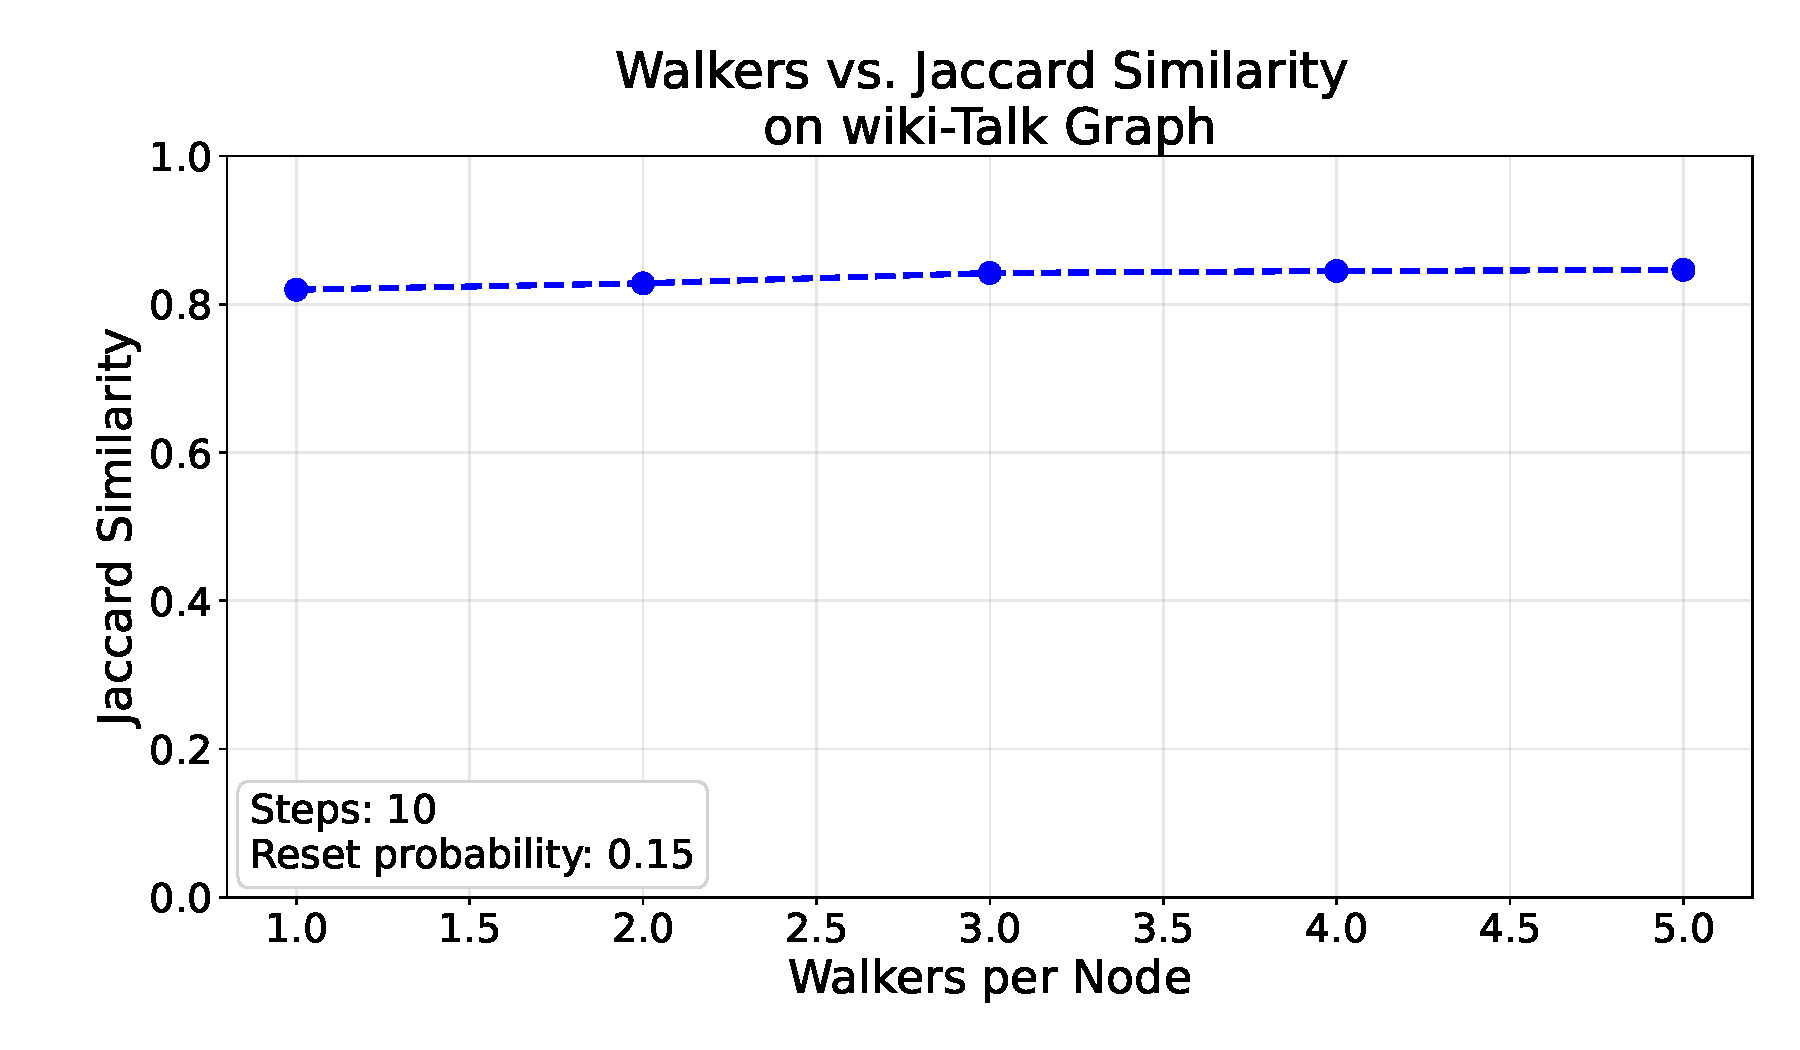
\includegraphics[width=\linewidth]{images/plots/wiki-Talk/accuracy_plots_wiki_talk.pdf}
        \caption{wiki-Talk}
        \label{fig:wikirun}
    \end{subfigure}\hfill
    \begin{subfigure}[t]{0.5\linewidth}
        \centering
        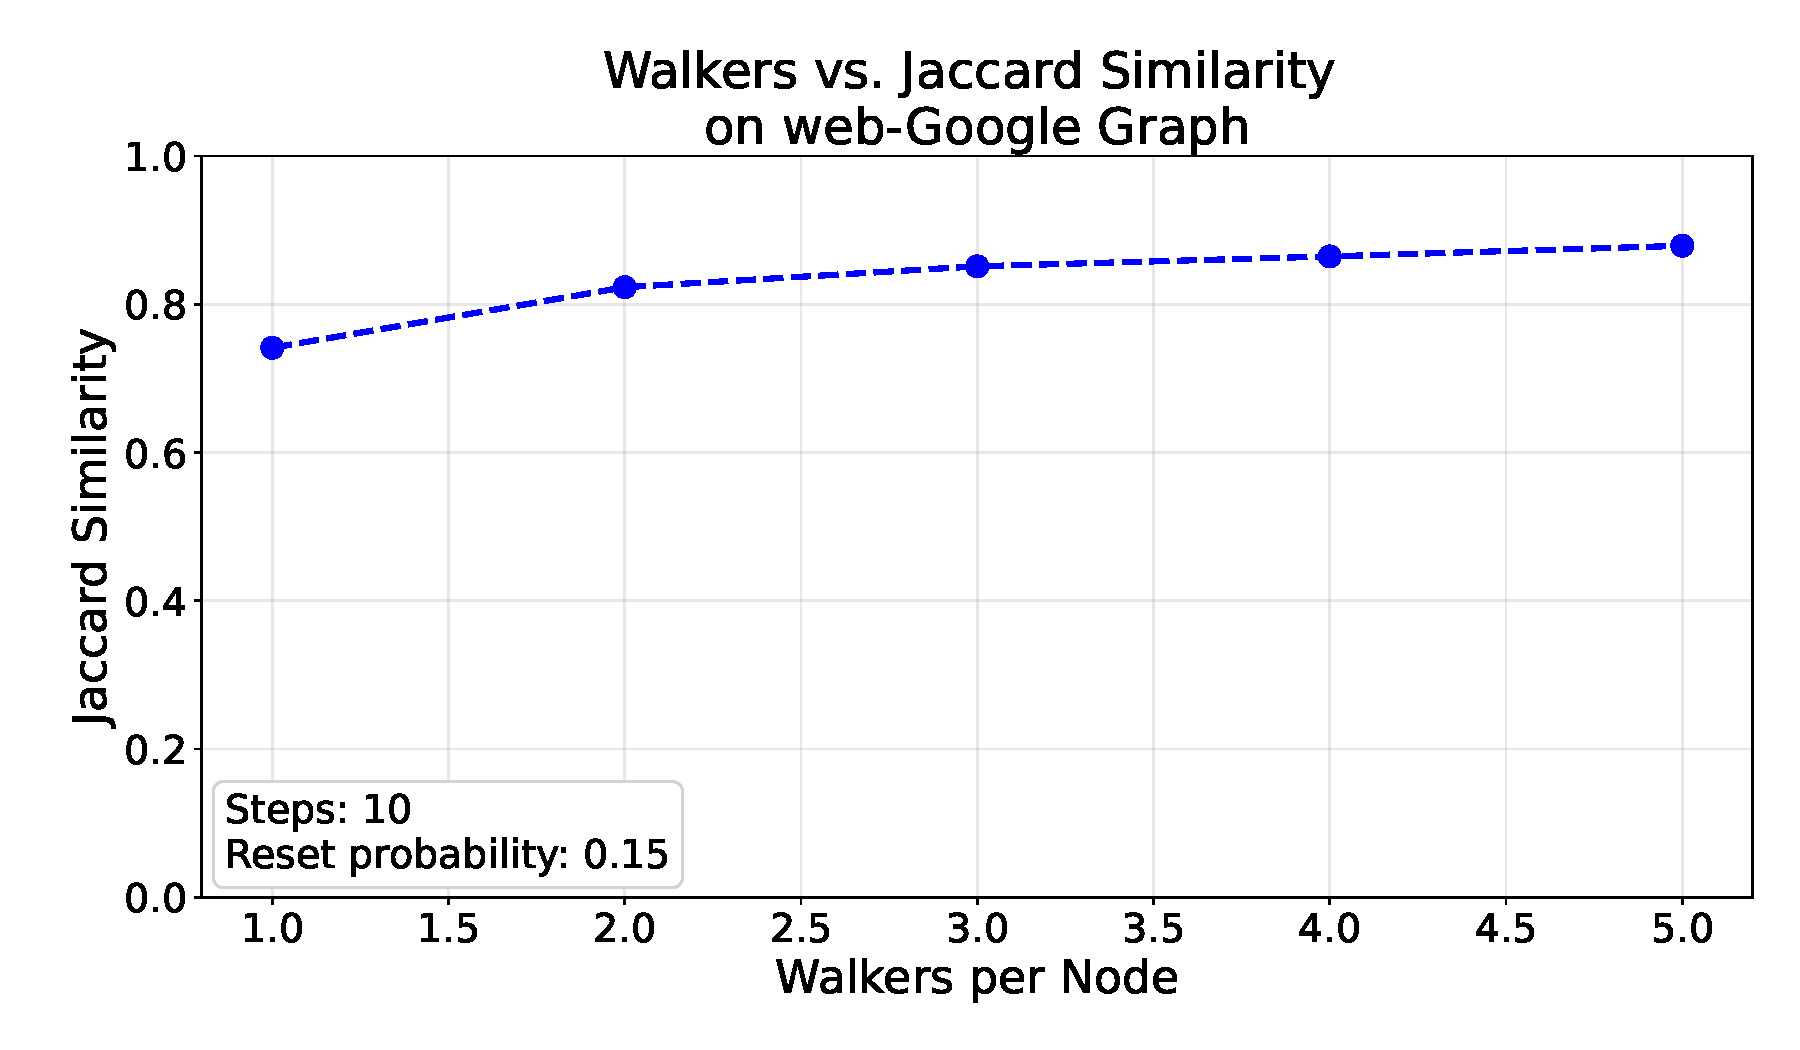
\includegraphics[width=\linewidth]{images/plots/web-Google/accuracy_plots_web_google.pdf}
        \caption{web-Google}
        \label{fig:wikigibhrs}
    \end{subfigure}
    \caption{Accuracy on real-world graphs}
    \label{fig:wiki-comparison}
\end{figure}








\subsection{Discussion}

The presented results in the previous section show that the Monte Carlo approach is a valid alternative to the standard PageRank implementation in memory constrained environments. This section discusses the findings across performance, cost and accuracy metrics to address the central research question: Is Monte Carlo PageRank an alternative to standard PageRank methods that is able to operate in a memory constraint environment while keeping acceptable performance and accuracy?\par

The experiments show that Monte Carlo PageRank is able to successfully compute rankings in memory constrained environments. Moreover, it achieves acceptable performance and accuracy. Monte Carlo PageRank operates on 450 MiB across all graph sizes and structures while GraphX requires 2-8 MiB on the same graphs. Surprisingly, the low memory configurations don't compromise performance of the Monte Carlo method. GraphX in contrast, suffers of severe performance issues on low memory configurations and large graphs even with higher resources. The relatively high accuracy between 75\% and 90\%, depending on the walker configuration, proves that Monte Carlo PageRank not only performs on limited memory but also delivers high quality results. In cases where GraphX is not able to operate, this simply gives the choice between getting an approximate result or not getting one at all. Additionally, the cost analysis supports the advantages that directly imply lower operational costs and more predictable behavior even with 20 million nodes. \par

Monte Carlo PageRank is ideal for applications where approximate rankings are sufficient such as recommendation systems or web search engines. The method's accuracy can easily be tuned based on the accuracy requirements. When configuring a minimal number of walkers an accuracy between 75\% and 83\% can be reached and up to 90\% with a higher walker configuration. \par  

However, Monte Carlo PageRank also introduces limitations that need to be considered. One of the main disadvantages is the instability across rankings due to the methods randomness. Therefore, multiple runs have to be done in case a stable ranking is required. Moreover, on larger synthetic graphs, where enough memory is configured, the GraphX method has lower runtimes compared to Monte Carlo PageRank. This implies that Monte Carlo PageRank is not universally superior regarding performance. Additionally, applications where rankings impact critical decisions, still need standard iterative PageRank methods that deliver exact results as approximate methods can not guarantee high precision. \par

Another aspect of this thesis that needs to be discussed is the experimental setup. Although it is systematic and reproducible, it presents some disadvantages. The setup consists of a Spark Cluster with 8 cores representing a relatively small distributed system compared to many production deployments. Moreover, the real-world graphs used in the experiments did not exceed 2.4 million nodes and for synthetic graphs only sizes up to 20 million nodes were tested. This is below the scale of many web graphs. However, the results are still valuable since they capture the scalability patterns of both PageRank methods. Additionally, the steps configuration was kept at a constant value of 10 steps per walker, which proved effective during the experiments but could be adapted to further improve Monte Carlo PageRank.\par

Despite the limitations Monte Carlo PageRank serves as a serious cost efficient alternative to standard methods. The approach successfully manages to do large scale graph analytics in memory constraint scenarios with little accuracy and performance trade-offs.



\subsubsection{Trade-offs}
\subsubsection{Experimental setup: realistic?}
\subsubsection{Monte Carlo Approach: good Alternative?}
% Interpret results and explain when your approach is advantageous.
